\documentclass[a4paper]{article}
\usepackage[utf8]{inputenc}
\usepackage{graphicx}
\usepackage[export]{adjustbox}
\usepackage{geometry}
\usepackage{titling}
\usepackage{fancyhdr}
\usepackage[]{todo}
\usepackage{acronym}
\usepackage{xcolor}
\usepackage{pgfgantt}
\usepackage{amsmath}
\usepackage{biblatex}
\usepackage{cleveref}
\usepackage{tikz}

\usetikzlibrary{shapes.geometric, arrows}

\tikzstyle{component} = [rectangle, rounded corners, minimum height=1cm, minimum width=3cm, text centered, draw=black]
\tikzstyle{arrow} = [thick,->,>=stealth]

\geometry{
outer=20mm,
inner=20mm,
top=20mm,
bottom=40mm}

\pagestyle{fancy}
\fancyhead[L]{Philip Nys}
\fancyhead[C]{C2PA Live Streaming}
\fancyhead[R]{Abstract}

\author{Philip Nys}

\title{Abstract - Master's Thesis\\Proof of Concept: Live Streaming C2PA-signed Content}

\newcommand{\code}[1]{\colorbox{lightgray}{\texttt{#1}}}

\begin{document}

\maketitle

\pagenumbering{roman}

\section{Motivation}

Nowadays it is getting harder and harder to distinguish real, unaltered content from manipulated and automatically generated content. The tools for editing content are getting more and more accessible and easier to use and there are even many so called "GenAI" tools which are able to create more and more convincing content from a simple text prompt.

This has lead to founding of the Coalition for Content Provenance and Authenticity (C2PA) in February 2021 \footnote{C2PA Founding Press Release \url{https://c2pa.org/post/c2pa_initial_pr/}} by large players in the industry: Adobe, Arm, BBC, Intel, Microsoft and Truepic, with the goal to establish a standardized method of signing a wide range of content with metadata to verify its authenticity, origin, alterations and more.

One type of content that hasn't yet been explored in depth is live streaming fragmented media. I hereby propose a Proof of Concept (POC) for C2PA-signed live content, implement it in a testbed and analyze its effectiveness.

\section{Overview C2PA}

The technical specifications \footnote{C2PA Specification \url{https://c2pa.org/specifications/specifications/2.0/specs/C2PA_Specification.html}} describe the data structures, signing and verification processes, supported content types and more.

The primary component of the signature is the C2PA Manifest, which gets embedded into the content in the signing process. This Manifest consists of the Claim Signature, a digital signature of the Claim, the Claim, a manipulation-proof data structure containing all information regarding the asset, and a number of Assertions, which describe the authenticity of the asset in form of data about the creation, the steps of changes that has been made to it, metadata about the device and people having been part in making of this asset and many more.

In the current specifications there is already a wide range of formats supported, including PDF, JPEG, GIF, PNG, BMFF and more. The type of embedding varies depending on the target file, for example in case of BMFF, the relevant type for fragmented content, the Manifest is encoded into a BMFF Box "uuid" (the box is not called "c2pa" as expected, because Chromium-based browsers refuse playback of content containing unspecified BMFF boxes) and in this Box the Manifest data is structured in the JPEG universal metadata box format (JUMBF).

There is an official open source implementation of the specification in Rust in form of the \textit{c2pa-rs} crate \footnote{c2pa-rs \url{https://github.com/contentauth/c2pa-rs}}, providing an application programming interface (API). Additionally, there is a command line interface (CLI) tool, called \textit{c2patool} \footnote{c2patool \url{https://github.com/contentauth/c2patool}}, which provides an user interface to the API to sign content in a terminal.

\section{Goals - Proof of Concept}

The goal of this thesis is to implement a POC testbed for live streaming fragmented media and evaluate its feasibility. The proposed setup of the testbed is shown in \Cref{fig:setup}. The testbed will be made up of four components. 

The process begins with the Producer component and will be an FFmpeg \footnote{FFmpeg \url{https://www.ffmpeg.org/}} script, which will generate an MPEG-DASH live stream from an input video file by endlessly loop through it. The output of this script will point to an HTTP output.

The second component will be the recipient of the HTTP output. This component will be integrated into the \textit{c2patool} by adding a CLI flag to make the tool run as a HTTP server to receive the fragments generated by the Producer. These fragments will then be signed with a C2PA Manifest. Once the signing process is completed the signed fragments will then be forwarded to a CDN.

The Content Delivery Network (CDN) is the third component and represents a simple HTTP server which receives the signed live stream (ingest) and distributes them to clients for consumption (digest).

The final component is the Consumer which is a web-based client using \textit{dash.js} \footnote{dash.js \url{https://github.com/Dash-Industry-Forum/dash.js}} to request and play the signed stream. Additionally, the client will also verify that the received fragments are valid.

This setup will mimic a close to reality content production, where some kind of content is produced (here represented by a static video file), this then gets encoded into a fragmented live stream (here using FFmpeg). Then there is the added component of signing the content with a C2PA Manifest to prove authenticity. Ideally, these two steps would be later merged into a single step. Finally, the produced stream would be published to and hosted on a large CDN to have it available for consumption.

The big task of this setup is how to optimize the signing process. The API currently only allows to sign a complete set of fragmented BMFF files. Since a live stream is continuously generating new fragments, for every new fragment (usually roughly every two seconds) this would require the re-signing of the entire live stream up until the newly created fragment, multiplied by every available track. On top of that all fragments would also be needed to be published to the CDN anew.

\begin{figure}
    \centering
    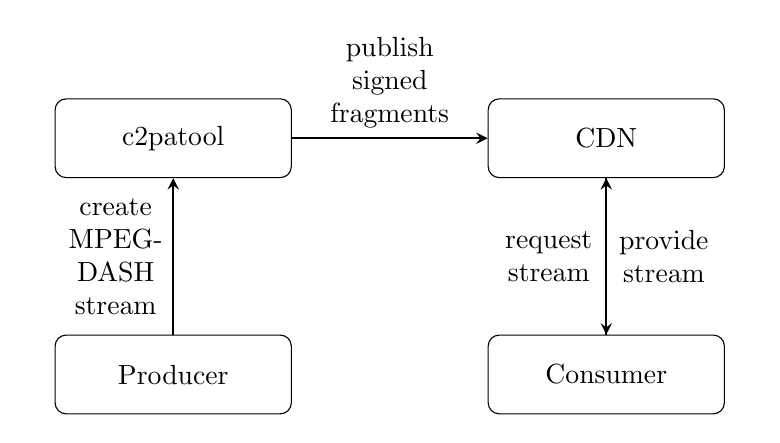
\begin{tikzpicture}[node distance=2cm]
        \node (producer) [component] {Producer};
        \node (c2pa) [component, above of=producer, yshift=1cm] {c2patool};
        \node (cdn) [component, right of=c2pa, xshift=3.5cm] {CDN};
        \node (consumer) [component, below of=cdn, yshift=-1cm] {Consumer};
    
        \draw [arrow] (producer) -- node[anchor=east, text width=2cm, text centered, xshift=0.4cm] {create MPEG-DASH stream} (c2pa);
        \draw [arrow] (c2pa) -- node[anchor=south, text width=2cm, text centered] {publish signed fragments} (cdn);
        \draw [arrow] (consumer) -- node[anchor=east, text width=2cm, text centered, xshift=0.4cm] {request stream} (cdn);
        \draw [arrow] (cdn) -- node[anchor=west, text width=2cm, text centered, xshift=-0.4cm] {provide stream} (consumer);
    \end{tikzpicture}
    \caption{Proof of Concept Testbed Setup}
    \label{fig:setup}
\end{figure}

\section{Time Schedule} 

A visual representation of the following schedule is depicted in \Cref{gantt:timeplan}.

I plan on having the proposal to be accepted by the end of January/early February. In the mean time I will begin with the setup of the basic testbed structure. This step will include the creation of an customizable FFmpeg script acting as the Producer, the extension of the \textit{c2patool} by a CLI flag to make is able to receive an MPEG-DASH live stream using HTTP and forwarding fragments, the implementation of a simple HTTP setup to act as the CDN and finally a simple webpage that can play the CDN-hosted live stream using \textit{dash.js}. I am expecting this step to take no more than four weeks.

In parallel to the initial setup I will begin writing the first draft of the thesis.

Next, I will begin work on the signing process. Beginning with a simple test to see how this setup runs without any changes to the existing API. However, I am expecting this to become very computationally expensive the longer the live stream is running. Then I will look into optimizing this process. This step will likely be the bulk of the entire thesis and I am estimating this to take between eight and twelve weeks.

Once the live stream is being signed and can be played by the Consumer, I will implement a client-side verification of the C2PA Manifests by hooking into the event listeners of \textit{dash.js} to inspect the received fragments, parse the C2PA "uuid" BMMF Boxes from them and perform the verification in accordance to the specifications. I have planned between two and four weeks for this step, depending on how long the previous optimization step takes.

Similarly, I have planned the same amount of time for the evaluation to measure the performance impact of signing a live streaming before publishing and possibly more if time permits.

I aim to conclude the first draft in conjunction with the evaluation to be able to sync-up with my supervisors to discuss last changes needed to finalize the thesis to submit the results by the end of the six months at the end of July.

\begin{figure}[t]
    \begin{center}
        \begin{ganttchart}[
            y unit title=0.4cm,
            y unit chart=0.5cm,
            vgrid,hgrid, 
            title label anchor/.style={below=-1.6ex},
            title left shift=.05,
            title right shift=-.05,
            title height=1,
            progress label text={},
            bar height=0.7,
            group right shift=0,
            group top shift=.6,
            group height=.3
        ]{1}{28}
            %labels
            \gantttitle{January}{4} 
            \gantttitle{February}{4} 
            \gantttitle{March}{4} 
            \gantttitle{April}{4} 
            \gantttitle{May}{4} 
            \gantttitle{June}{4}
            \gantttitle{July}{4} \\
            %tasks
            \ganttbar{Proposal}{3}{5} \\
            \ganttbar{Testbed Setup}{5}{8} \\
            \ganttbar{First Draft}{7}{24} \\
            \ganttbar{Optimize Signing}{9}{20} \\
            \ganttbar{Verification}{19}{22} \\
            \ganttbar{Evaluation}{21}{24} \\
            \ganttbar{Finalize Thesis}{25}{26} \\
            \ganttbar{Submit Thesis}{27}{28}
        \end{ganttchart}
    \end{center}
    \caption{Time Schedule}
    \label{gantt:timeplan}
\end{figure}

\end{document}